\documentclass[a4paper,twoside]{report}

\usepackage[utf8]{inputenc}
\usepackage[T1]{fontenc}
\usepackage[francais]{babel}
\usepackage{setspace}
\usepackage{layout}
\usepackage{amsmath}
\usepackage{amssymb}
\usepackage{mathrsfs}
\usepackage{graphicx}



\renewcommand{\contentsname}{Sommaire}
\pagestyle{headings}



\title{Rapport projet long\\Équipe HAL9000}
\author{Hamelain Christian, Hasan Pierre-Yves, Gaspart Quentin, Trestour Fabien}


\begin{document}


    \setcounter{tocdepth}{1}


    \maketitle


    \tableofcontents


    \part{Introduction}

        \section[Contexte]{Contexte du projet}

            CentraleSupélec propose à  ses étudiants en deuxième année de participer
            à  des projets longs qui se réalisent en équipe, tout au long de l'année sur un thême mêlant plusieurs compétences que l'ingénieur se doit de posséder.

            Dans notre cas, c'est l'élaboration de réseaux neuronaux et les méthodes de Deep Learning que 12 éléves ont étudié, répartis en 3 groupes, dont HAL9000.

            Ce rapport présente les avancement de ce dernier groupe sur le sujet tout au long de l'année.


        \section{Présentation du sujet}

            Ce projet aborde le sujet du Deep Learning. Cette méthode spécifique de machine learning est dérivée du concept de réseau de neurones.

            Les réseaux de neurone sont une modélisation simple du fonctionnement cérébral
            à  l'échelle cellulaire. Cette approche a vu le jour avec les études de McCulloch et Pitts dès la fin des années 50. Malgré certains écueils dans les années 70, l'approche connexioniste des réseaux de neurones a su se développer et devenir un sujet de recherche populaire dans les dernières années, notament grâce aux capacités d'adaptabilité et de généralisation de ces réseaux qui en font d'excellents candidats pour des applications telles que la reconnaissance d'image ou la classification.


        \section[Déroulement]{Déroulement du projet}

            Tout d'abord, il s'agissait pour nous de comprendre le fonctionnement de ces structures et commencer à  coder des structures élémentaires afin de comprendre les enjeux du machine learning. Nous avons pour cela travaillé avec la base de données MNIST de Yves LeCun et en JAVA. Afin de travailler en groupe de manière efficace, nous avons aussi utilisé l'outil GIT.

            Par la suite nous nous sommes interessés aux architectures profondes, chaque groupe se penchant sur une architecture spécifique. Notre équipe s'est en particulier intéressée aux machines de Boltzmann, en commenà§ant par les machines de Boltzmann restreintes (RBM), puis la structure de Deep Learning associée.

            Cette étude a été encadrée par Joanna Tomasik et Arpad Rimmel, enseignants à  CentraleSupélec, campus de Gif-sur-Yvette.



    \part[Le Perceptron]{Première approche du problème : le Perceptron}


        \chapter{Architecture d'un perceptron}

            \section{Introduction}

                Ici, l'objectif était la reconnaissance des caractères de la base de données MNIST grâce à  un perceptron.

                Le perceptron fait partie des architectures de réseaux neuronaux les plus simples. Son étude nous a donc permis de s'introduire à  la problématique du machine learning avant d'approfondir en étudiant des structures plus complexes.


            \section{La brique de base : le neurone}

                Le neurone est le composant élémentaire des réseaux neuronaux. Il est une modélisation du fonctionnement des neurones du systême nerveux humains.

                Chaque neurone reà§oit un signal via une entrée, qui correspond aux dendrites des systèmes biologiques. Le neurone prend en compte la valeur de toutes ses entrées et en déduit la valeur de sortie. Cette sortie est ensuite propagée par le biais d'un axone vers un autre neurone.\\

                \begin{figure}
                    \begin{center}
                        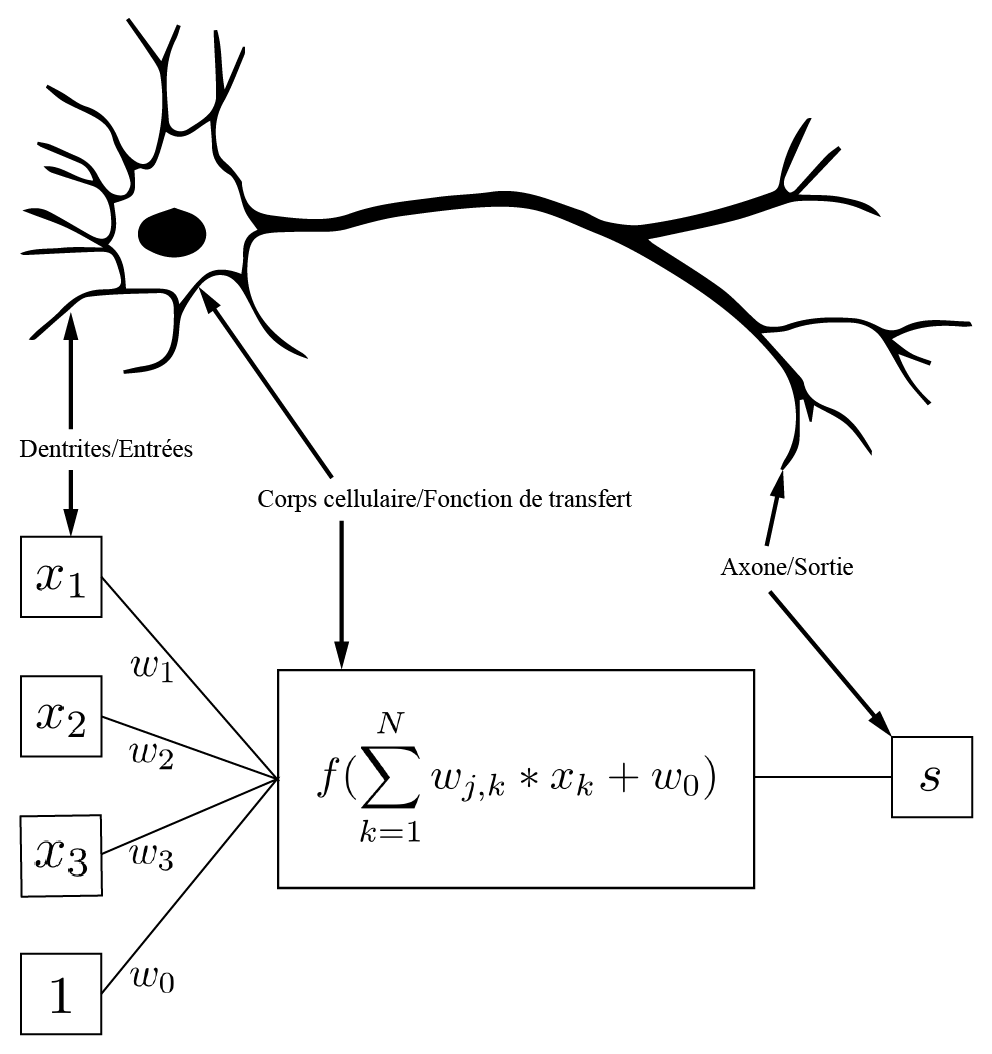
\includegraphics[width=200pt]{Images/neurone-01.png}
                    \end{center}
                    \caption{Analogie entre neurone biologique et neurone formel.}
                \end{figure}

                La sortie du j\textsuperscript{ième} neurone est donnée par la formule :

                \begin{equation}\label{eqNeur}s_{j}(x)=f(\sum_{k=1}^{N} w_{j,k}*x_{k}+w_{0})\end{equation}

                où:

                \begin{itemize}
                    \item $s$ est la valeur de la sortie
                    \item $f$ est la fonction d'activation.
                    \item N est la dimension du vecteur d'entrée.
                    \item $w_{j,k}$ est la k\textsuperscript{ième} composante du vecteur de poids $w_{j}$ du j\textsuperscript{ième} neurone. $w_{0}$ est le biais du neurone. Cette valeur correspond au poids d'une entrée fictive valant toujours 1.
                    \item $x_{k}$ est la k\textsuperscript{ième} composante du vecteur d'entrée $x$.\\
                \end{itemize}

                L'entrée $x$ est un vecteur défini par un ensemble de caractéristiques que l'on choisit pour représenter les données d'entrées. Dans le cas d'une image par exemple, ce vecteur d'entrée peut être composé de la valeur de tous les pixels de l'image. D'autres représentations moins triviales peuvent être choisies afin de réduire la quantité d'information à  traiter et de s'approcher au mieux des données signifiactives de la problématique traitée.\\

                La fonction d'activation permet de définir le comportement du neurone. Selon la définition de cette fonction on aura une sortie à  valeurs discrètes ou continues, centrées en 0 ou en 0,5. Le choix de la fonction est donc étroitement lié avec le problème à  traiter.
                Il existe différents types de fonctions d'activation. Parmis les plus utilisées figurent:
                \begin{itemize}
                    \item La fonction échelon
                    \begin{equation}
                        f(x)=\mathbf{1}_{\mathbb{R}^{*}_{+}}
                    \end{equation}
                    \item Les fonctions linéaires
                    \begin{equation}
                        f(x)=\alpha*x+\beta
                    \end{equation}
                    \item La fonction sigmoïde
                    \begin{equation}
                        f(x)=\frac{1}{1+e^{-\lambda*x}}
                    \end{equation}
                    \item La fonction tangente hyperbolique
                    \begin{equation}
                        f(x)=\frac{e^{x}-e^{-x}}{e^{x}+e^{-x}}
                    \end{equation}
                \end{itemize}

                Le vecteur de poids du j\textsuperscript{ième} neurone représente la pondération de chacune des entrées de ce neurone. C'est ce paramètre qui permet de modifier le réseau de neurone sans avoir à  modifier son architecture. Toutes les propriétés d'un réseau neuronal sont donc issues de ce vecteur de pondération et de ses variations.


            \section{Organisation des couches}

                Il existe de nombreuses architectures de réseau de neurone. Elles peuvent être récurrentes ou non, entièrement connectées ou seulement partiellement, organisées en couches, ... De nombreuses propriétés permettent de caractériser une architecture de réseau de neurone.

                Le Perceptron est un modèle assez élémentaire de réseau. Il est constitué en couches totalement connectées.

                On peut distinguer trois types de couches : la couche d'entrée, les couches cachées et la couche de sortie.\\

                La couche d'entrée est assez élémentaire. C'est tout simplement une couche dont la valeur sera le vecteur d'entrée $x$. Cette couche doit donc être constituée d'autant de neurones que le vecteur d'entrée a de dimensions. Les neurones de cette couche ont pour fonction d'activation l'identité.\\

                Les couches cachées sont celles qui effectuent les calculs. Les principales propriétés du réseau sont héritées de cet empilement de couches. On comprend alors mieux l'intérêt actuel pour le Deep Learning, c'est-à -dire l'apprentissage des réseaux avec un grand nombre de couches cachées.
                Le nombre de neurones dans chaque couche et les fonctions d'activation utilisées par les neurones sont choisies par le concepteur du réseau selon le problême traité par le réseau.\\

                Afin d'expliciter l'importance de l'architecture du réseau, abordons l'exemple usuel du ou exclusif.

                Essayons de réaliser avec un unique neurone la fonction logique XOR. Ce neurone aura deux entrées $x_{1}$ et $x_{2}$ à  valeurs dans \{0;1\} et une sortie $s$, elle aussi à  valeurs dans \{0;1\}. On prendra comme fonction d'activation la fonction de Heaviside, c'est à  dire $\mathbf{1}_{\mathbb{R}^{*}_{+}}$. Ce neurone aura par conséquent un fonctionnement totalement binaire. Il s'agit donc ici de déterminer les pondérations $w_{1}$ et $w_{2}$, respectivement associées aux entrées $x_{1}$ et $x_{2}$, qui conviennent pour obtenir en sortie la valeur $x_{1}\oplus x_{2}$.\\

                Pour un tel problème, le neurone agit comme un séparateur linéaire de l'espace des entrées. L'équation de la droite séparant le demi-espace définit par $s=0$ de celui définit par $s=1$, découle alors directement de l'équation \ref{eqNeur}:

                \begin{equation}w_{2}*x_{2}+w_{1}*x_{1}+w_{0}=0\end{equation}

                On constate ici l'intérêt du biais, qui permet de réaliser des séparations affines de l'espace des entrées et pas seulement des fonctions linéaires.

                Les limites d'un neurone seul sont alors évidentes : toutes les séparations de l'espace des entrées ne sont pas affine, et le cas du XOR en est déjà  une illustration.\\

                Il est alors nécessaire d'introduire la structure de réseau. En prennant une couche d'entrée, une couche cachée et une couche de sortie, respectivement composées de deux, deux et un neurone, on peut contourner le problème sus-cité. Cette structure permet en fait de générer deux séparations de l'espace des entrées.

                La séparation que l'on cherche à  effectuer est en effet de la forme:

                \begin{equation}
                    f(x_{1},x_{2})=0 \Leftrightarrow
                    \left\{
                        \begin{array}{r c l}
                        x_{1}+x_{2}-0,5 &<& 0\\
                        x_{1}+x_{2}-1,5 &>& 0
                        \end{array}
                    \right.
                \end{equation}

                On obtient ainsi directement les valeurs de poids désirées grâce à  ces équations:
                \begin{equation}
                    blablabla
                \end{equation}

                Ce premier exemple simpliste manifeste donc la nécessité d'adapter la structure du réseau au problème traité.\\

                De manière plus générale, le nombres de neurones du réseau fait varier le nombre de poids du réseau, et donc la capacité du réseau à  séparer des ensembles multiples et complexes. Ainsi, un réseau sous-dimensionné mêne à  des résultats pas assez précis et un réseau sur-dimensionné mène à  du sur-apprentissage. On a donc environ la loi suivante:
                \begin{equation}
                    N<\frac{1}{10}*T*dim(s)
                \end{equation}
                \begin{itemize}
                    \item $N$ est le nombre de neurones dans le réseau.
                    \item $T$ est le nombre de vecteurs de la base d'apprentissage.
                    \item $s$ est le vecteur de sortie.
                \end{itemize}

                De plus, le nombre de neurones dans une couche doit être de moins de trois fois celui de la couche précédente.\\

                Ces deux approximations donnent donc une première idée de la structure à  adopter pour un réseau de neurones.



        \chapter{Algorithmes d'apprentissage}

            \section{salut}

                123


            \section{c'est cool}


        \chapter{La base MNIST}

        \chapter{Influence des paramètres sur l'apprentissage}




    \part[Machines de Boltzmann]{Approfondir le sujet : les machines de Boltzmann.}

        \chapter{Introduction}

            Les réseaux de Boltzmann sont des réseaux qui ont un fonctionnement
            particulier que nous allons présenter dans ce chapitre. Les machines de
            Boltzmann constituent des réseaux neuronnaux. La prinipale différence entre
            les réseaux neuronnaux comme les réseaux neuronnaux de convolution (CNN) et
            les  réseaux de Boltzmann va être le fait qu'un réseaux de Boltzmann n'est
            pas \textit{feed-forward} ; comme l'était le perceptron, présenté dans ce
            rapport.

            Ce rapport traitera d'abord des machines de Boltzmann restreintes en les
            présentant et en expliquant les lois qui régissent leur fonctionnement pour
            ensuite s'intéresser aux Réseaux de Boltzmann Profond.

        \chapter{Les machines de Boltzmann restreintes}

            Les machines de Boltzmann restreintes, ou RBM, ont d'abord été
            pensées par P. Smolensky (1986) mais réellement mise en oeuvres et
            étudiées par G.
            Hinton(2006). Nous allors présenter dans cette partie leur constitution et
            leurs fonctionnement.

            \section{Principe}

                Les RBM sont des réseaux neuronnaux et sont donc constituées de d'entité que
                l'on nommera neurone qui possède une fonction d'activation, qui donne une
                probabilitéde l'activation du neurone, et de synapses qui relient ces neurones.

                Une RBM possède deux couches de neurones, une que l'on appellera couche
                visible et une autre que l'on appellera couche cachée. La couche visible
                correspond à l'entrée de notre réseau, ce sont les neurones de la couches
                d'entrée auxquels ont va assigner les exemples de notre jeu de données pour
                entrainer le réseau. Au sein d'une même couche, aucun neurone n'est relié à un
                autre, c'est ce caractère restreint qui donne sa particularité et son nom à ce
                type de réseau de Boltzmann. Par contre un neurone de la couche visible
                (respectivement cachée) est connecté à tous les neurones de la couche cachée
                (respectivement visible). 

                On forme ainsiun graphe, les particularités de la machine restreintes font que
                l'on a 

                A expliquer : MRF et les propriété --> chaine de Markov
                Particularité et donc convergence --> contrastive divergence.

                La particularité de ce réseau est donc le fait qu'il n'est pas
                \textit{feed-forward}, même si l'on considère la couche cachée comme entrée du
                réseaux.



        \chapter{Les Deep Belief Networks}



        \chapter{Aller plus loin}

            \section{La visualisation des spectres du réseau}

                Lors du développement de la RBM, nous avons étés confrontés au problème de la quantification de l'apprentissage. Comment savoir si oui ou non le réseau s'adapte aux exemples qu'on lui a présenté ?\\

                Suite à l'absence de réelle mesure de cette notion, l'idée nous est venue d'implémenter une mesure bien plus qualitative du phénomène : l'objectif était de visualiser l'importance que le réseau accorde à chaque pixel de l'image.\\

                Dans le cas de la RBM, cela correspond tout simplement à l'ensemble des pondérations des connections entre la couche visible et la couche cachée du réseau. Ainsi, à chaque neurone de la couche cachée, on peut associer une image correspondant aux dites pondérations. Ce sont ces images que l'ont qualifie de "spectres".

                Ces spectres représentent les caractéristiques que le réseau essaie de détecter dans une image pour y reconnaître un caractère. Selon le nombre de neurones dans la couche cachée, ces caractéristiques sont assez différentes. En effet, plus il y a de neurones cachés, plus le réseau pourra détecter de nombreuses caractéristiques précises, qui une fois assemblées formeront la représentation du caractère complet. Ces caractéristiques peuvent être, par exemple, des angles ou des boucles. A contrario, quand le réseau a peu de neurones cachés, ces spectres sont beaucoup plus proches de la forme "usuelle" du caractère associé. Ainsi, avec un seul neurone caché, on obtient très exactement la représentation d'un chiffre idéal pour ce réseau.\\

                L'intérêt d'une telle initiative est simple : utiliser l'intuition visuelle qu'on a des chiffres pour juger de la qualité de l'apprentissage.

                Au début de l'apprentissage, l'image sera exclusivement composée de bruit blanc, tandis qu'à la fin elle ressemblera au négatif d'un des exemples de la base de donnée (toutjours dans le cas d'un réseau à un seul neurone caché).


\end{document}
